\documentclass[11pt]{article}
\usepackage{graphicx}
\usepackage{hyperref}
\usepackage{natbib}
\usepackage{amsmath}

\setlength{\textwidth}{6.5in}
\setlength{\headheight}{0in}
\setlength{\textheight}{8.0in}
\setlength{\hoffset}{0in}
\setlength{\voffset}{0in}
\setlength{\oddsidemargin}{0in}
\setlength{\evensidemargin}{0in}

\title{PS3}
  
\author{Shihong Pan\\ \url{https://github.com/PSH-hub24/phys-ga2000}}


\begin{document}

\maketitle

\section{Q1}
Fig \ref{fig:Q1} shows the computation time scaled with $N$, using different methods. It is obvious that the scaling of the explicit function matches that of the $N^3$ curve.

\section{Q2}
Fig \ref{fig:Q2} shows the simulation results.

\section{Q3}
Fig \ref{fig:Q3} shows the simulation results.

\section{Q4}
The expectation and variance of the given exponential distribution are
\begin{equation}
    \mu_x = 1, \sigma^2_x = 1
\end{equation}
Then those of $y$ are
\begin{equation}
    \begin{aligned}
    \mu_y &= \frac{1}{N}\sum_{i=1}^N\mu_x=\mu_x=1 \\
    \sigma^2_y &= \frac{1}{N^2}\sum_{i=1}^N\sigma^2_x=\frac{1}{N}
    \end{aligned}
\end{equation}
Fig \ref{fig:Q4LargeN} shows the change in the distribution of $y$ as $N$ increases. Fig \ref{fig:Q4Moments} plots the mean, variance, skewness, and kurtosis of the distribution of $y$ as function of $N$. Fig \ref{fig:Q4OnePercent} shows an estimation of $N$ where the skewness and kurtosis have reached about 1\% of their value for $N=1$.


\begin{figure}[b!]
\centering
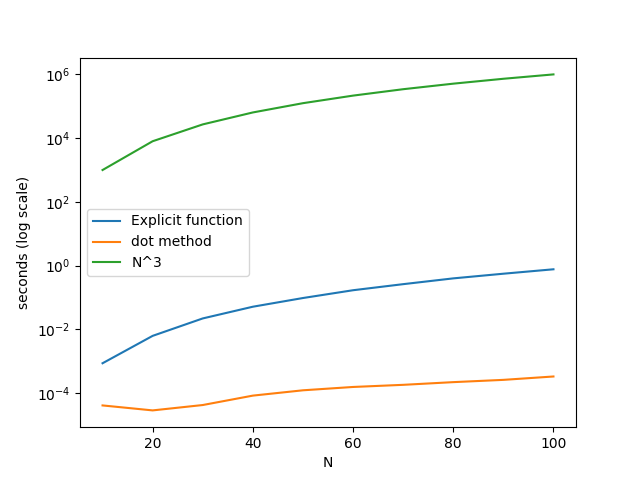
\includegraphics[width=0.6\textwidth]{Computational Physics/ps3Figures/q1(log_scale).png}
\caption{The computation time (in log scale) of computing $N\times N$ matrix multiplication, using an user-defined explicit function and the dot() method, compared to the $N^3$ scaling.}
  \label{fig:Q1}
\end{figure}

\begin{figure}[b!]
\centering
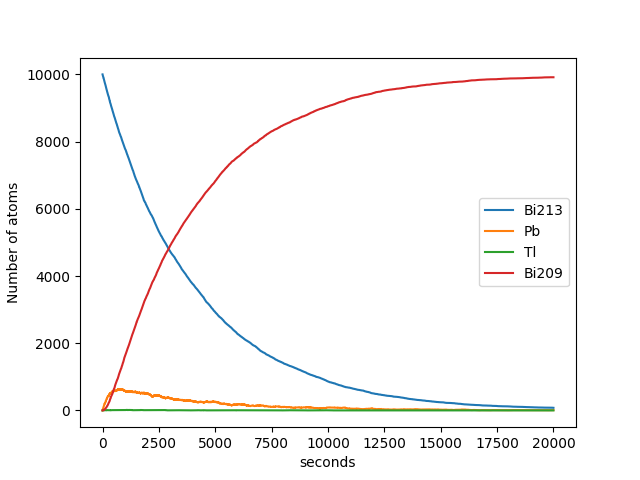
\includegraphics[width=0.6\textwidth]{Computational Physics/ps3Figures/q2.png}
\caption{Decay simulation. The figure plots the number of Bi213, Pb209, Tl209, and Bi209 atoms over 20000 seconds.}
  \label{fig:Q2}
\end{figure}

\begin{figure}[b!]
\centering
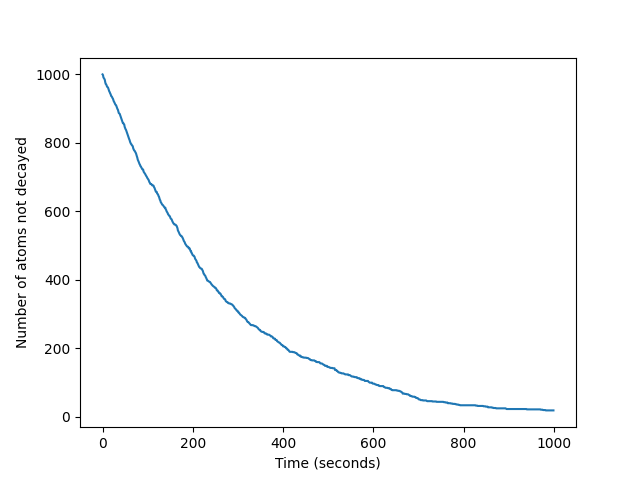
\includegraphics[width=0.6\textwidth]{Computational Physics/ps3Figures/q3.png}
\caption{Decay simulation. The figure plots the number of Tl208 atoms over 1000 seconds, using the transformation method to speed up the computation time.}
  \label{fig:Q3}
\end{figure}

\begin{figure}[b!]
\centering
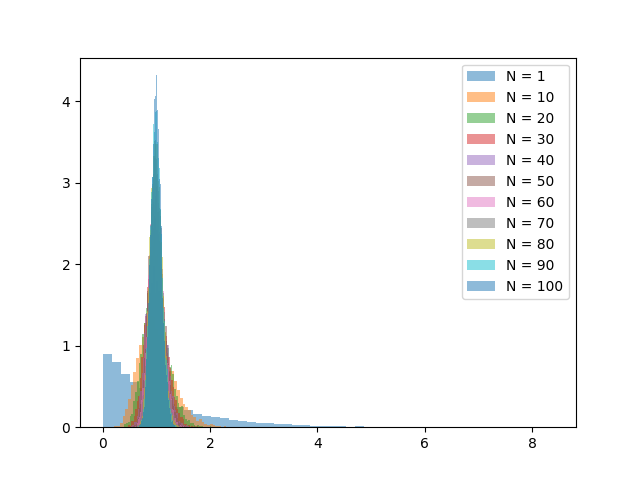
\includegraphics[width=0.6\textwidth]{Computational Physics/ps3Figures/q4LargeN.png}
\caption{The distribution of $y$ for large $N$.}
  \label{fig:Q4LargeN}
\end{figure}

\begin{figure}[b!]
\centering
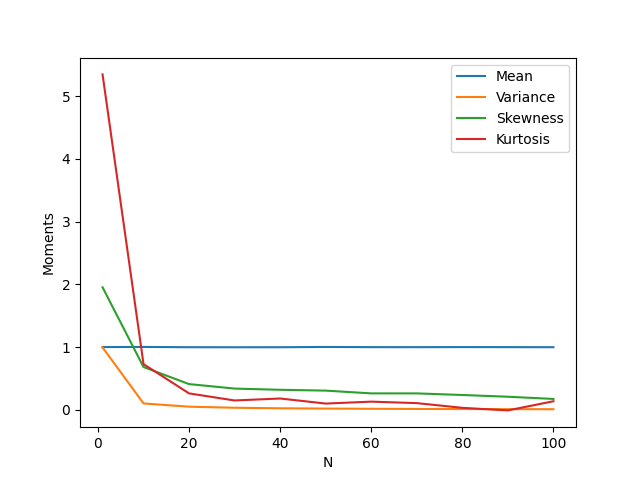
\includegraphics[width=0.6\textwidth]{Computational Physics/ps3Figures/q4Moments.png}
\caption{The mean, variance, skewness, and kurtosis of the distribution of $y$ as function of $N$.}
  \label{fig:Q4Moments}
\end{figure}

\begin{figure}[b!]
\centering
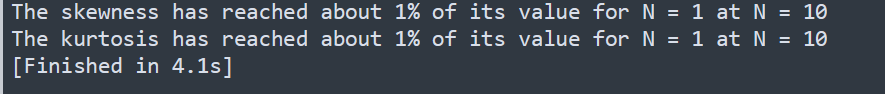
\includegraphics[width=0.6\textwidth]{Computational Physics/ps3Figures/q4OnePercent.PNG}
\caption{Estimation of the value of $N$ where the skewness and kurtosis have reached about 1\% of their value for $N=1$.}
  \label{fig:Q4OnePercent}
\end{figure}

\bibliographystyle{apj}
\bibliography{example}

\end{document}

 
 
